\section{Data Analysis}\label{section:data_anal}
Data analysis is the act of analyzing, cleansing, manipulating, and modeling data in order to identify usable information, generate conclusions, and help decision-making processes~\cite{Book:sbrown_2014_transforming}.
In today's corporate world, data analysis plays an important part in making decisions more scientific and assisting firms in operating more efficiently. 

Data analysis has several dimensions and approaches, including a wide range of techniques known by various names and applied in a variety of business, science, and social science sectors~\cite{Book:pruneau_2017}.
Let's give some examples.
\ac{DM} is a type of data analysis technique that focuses on statistical modeling and knowledge discovery for predictive rather than purely descriptive purposes,
whereas \ac{BI} is a type of data analysis that focuses on aggregation and is primarily concerned with business information.
Furthermore, in statistical applications, Data analysis can be separated into descriptive statistics, \ac{EDA}, and \ac{CDA}~\cite{Book:doing_data_science}. 
\ac{EDA} is concerned with finding new features in data, whereas \ac{CDA} is concerned with validating or refuting current assumptions~\cite{Article:intro_to_data_analysis}.
Finally, predictive analytics focuses on the application of statistical models for predictive forecasting or classification,
while text analytics, applies statistical, linguistic, and structural techniques to extract and classify information from textual sources, a species of unstructured data.
All the aforementioned are examples of data analysis~\cite{Article:goodnight_2011_the}.

\subsection{Procedure for analyzing data}
\label{subsect:data_analysis_proc}
\begin{figure}[ht]
    \centering
    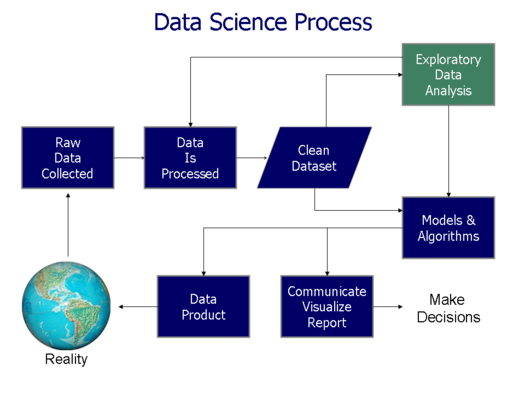
\includegraphics[width=0.9\textwidth]{Data_visualization_process_v1.png}
    \caption{Data science process flowchart (Source:~\cite{Book:doing_data_science})}
    \label{fig:data-science-flowchart}
\end{figure}
The term \textit{``analysis''} refers to the process of breaking down a whole into its constituent parts for closer evaluation.
Data analysis is the act of getting raw data and then transforming it into information that users can utilize to make decisions~\cite{Book:sbrown_2014_transforming}.
Data is gathered and processed in order to answer questions, test hypotheses, or refute theories.
Statistician \citeauthor{Article:future_of_data_tukey}, defined data analysis in 1961~\cite{Article:future_of_data_tukey}, as following:
\begin{quote}
    ``Procedures for analyzing data, techniques for interpreting the results of such procedures, ways of planning the gathering of data to make its analysis easier,
    more precise or more accurate, and all the machinery and results of (mathematical) statistics which apply to analyzing data.''
\end{quote}
There are various distinct phases that can be identified as show in Figure~\ref{fig:data-science-flowchart}, these are iterative in the sense that input from later phases may lead to further effort in earlier ones~\cite{Book:doing_data_science}.
Next, we are going to present them one by one, in a slightly more detailed manner, stressing that similar stages can be found in the \ac{CRISP} framework, which is used in \acl{DM}.

\subsubsection{Data Collection}
Data is collected from a broad variety of sources, like sensors in the environment, including traffic cameras, satellites, recording devices, etc. and
it may also be obtained through interviews, downloads from online sources, or reading documentation~\cite{Book:doing_data_science}.

\subsubsection{Data Processing}
Data, when initially obtained, must be processed or organized for analysis.
For instance, these may involve placing data into rows and columns in a table format (known as structured data) for further analysis, often through the use of spreadsheet or statistical software~\cite{Book:doing_data_science}.

\subsubsection{Data Cleaning \& Cleansing}
After it has been processed and structured, data may be missing, duplicated, or contain errors. Data cleaning will be essential as a result of challenges with the way data is entered and stored.
The process of detecting and correcting (or removing) corrupt or inaccurate records from a record set, table, or database is, indeed, known as data cleansing (or \textit{cleaning}),
and it entails identifying incomplete, incorrect, inaccurate, or irrelevant parts of the data and then replacing, modifying, or deleting the dirty or coarse data~\cite{Misc:2019_data_cleaning_wiki}.
The actual data cleaning workflow may include removing typographical errors and/or validating and correcting values against a known list of entities.

\subsubsection{\acl{EDA}}
Once the datasets are cleaned, they can then be analyzed.
\ac{EDA} is the first step toward building a model, since it is a critical part of the data science process, and also represents a philosophy developed by~\citeauthor{Article:future_of_data_tukey}
in contrast to \ac{CDA}, which concerns itself with modeling and hypotheses~\cite{Article:future_of_data_tukey}.
Indeed, in \ac{EDA}, there is no hypothesis and there is no model. The ``exploratory'' aspect means that your understanding of the problem you are solving, or might solve, is changing as you go.

The process of data exploration may result in additional data cleaning or additional requests for data; thus, the initialization of the iterative phases mentioned in the lead paragraph of this section.
Data visualization is also a technique used, in which the analyst is able to examine the data in a graphical format in order to obtain additional insights, regarding the messages within the data~\cite{Book:doing_data_science}.

\subsubsection{Modelling and algorithms}
Mathematical formulas or models (known as algorithms) can be applied to data to identify relationships between variables, such as correlation or causation~\cite{Book:pruneau_2017}.
In general, models can be created to evaluate a specific variable based on other variables in the dataset, with some residual error depending on the accuracy of the implemented model (e.g., $Data = Model + Error$)~\cite{Book:judd_1989_data_model}.

\subsubsection{Data product}
A data product is a computer application that takes data inputs and generates outputs, feeding them back into the environment.
As such it may be based on a model or algorithm. For instance, an application that analyzes data about customer purchase history, and uses the results to recommend other purchases the customer might enjoy~\cite{Book:doing_data_science}.

\subsubsection{Data visualization \& Communication}
Once data is analyzed, it may be reported in many formats to the users of the analysis to support their requirements~\cite{Article:intro_to_data_analysis}.
The users may have feedback, which results in additional analysis. As such, much of the analytical cycle is iterative, as stated before.
A company dashboard, for instance, that visualizes some \ac{KPIs}, is both a data product and a decision support system, with a nice user interface that allows  to access multiple visualization~\ref{section:grafana}.

\subsection{What is Data?}
\begin{table}[ht]
    \begin{tabularx}{\textwidth}{
            | >{\raggedright\arraybackslash} m{1.8cm}
            | >{\raggedright\arraybackslash} m{1.8cm}
            | >{\raggedright\arraybackslash} X
            | >{\raggedright\arraybackslash} X |}
        % \hline
        % \multicolumn{4}{|c|}{NOIR} \\
        \toprule
        \hfil\bfseries Variable & \hfil\bfseries Type(s) & \hfil\bfseries Description                                                            & \hfil\bfseries Examples                                                      \\
        \midrule
        Categorical             & Nominal                & Named categories with no implied order                                                & Blood groups, breed, gender, neuter status                                   \\
        ~                       & Ordinal                & Ordered categories where the differences between categories are not necessarily equal & Scoring systems, cancer staging, onset of disease (peracute, acute, chronic) \\
        \midrule
        Continuous              & Interval               & Equal distances between values, but the zero point is arbitrary                        & IQ, ordinal data with equal-appearing categories                             \\
        ~                       & Ratio                  & Above as for interval and a meaningful zero; data usually obtained by measurement     & Weight, age, temperature, blood pressure                                     \\
        \bottomrule
    \end{tabularx}
    \caption{NOIR system of classification of types of data (Source:~\cite{Article:intro_to_data_analysis})}
    \label{table:noir_sys}
\end{table}
We discussed at length about data in the previous subsection; certainly it is important that one have the ability to analyse and investigate data, but 
understanding data is an important prerequisite for being able to use it properly, and perhaps the single most important element.
Fortunately the NOIR system, commonly used, can help us. It defines the type of data as nominal, ordinal, interval or ratio as show in table~\ref{table:noir_sys}.

So we can confirm that valuable data is no longer only a collection of numbers and classified variables and
a strong data scientist needs to be versatile and comfortable dealing with a variety of types of data, including:
\begin{itemize}
    \item Traditional: numerical, categorical, or binary.
    \item Text: emails, tweets, New York Times articles.
    \item Records: user-level data, timestamped event data, log files.
    \item Complex: Geo-based location data (GIS), Network \& Images.
    \item Sensor data, my use-case (see Chapter~\ref{chapter:use_cases}).
\end{itemize}
% On how to deal with different types of data, it represents open research questions for the statistical and computer science community. 
% This is the frontier! Since some of these are open research problems, in practice, data scientists do the best they can, and often invent new methods as part of their work.

% \paragraph{Connection to the Scientific Method}
\subsection{Connection to the Scientific Method}
In both the data science process and the scientific method, not every problem requires one to go through all the steps, but almost all problems can be solved with \textit{some} combination of previously mentioned stages~\cite{Book:doing_data_science}.
In fact, We can think of the data science process as an extension of or variation of the scientific method:
\begin{itemize}
    \item Ask a question.
    \item Do background research.
    \item Construct a hypothesis.
    \item Test your hypothesis by doing an experiment.
    \item Analyze your data and draw a conclusion.
    \item Communicate your results.
\end{itemize}
As an example, if your end goal is a \textbf{data visualization} (which itself could be thought of as a data product), it's possible you might not do any machine learning or statistical modeling,
but you would want to get all the way to a clean dataset, do some \acl{EDA}, and then create the visualization. This has happened to me many times during my internship, as we will see in Chapter~\ref{chapter:use_cases}.

\paragraph{Data-driven context}
There are numerous areas in which data analysis shines, but in this text we will focus on one specific area: maintenance.
For complex systems such as airplanes, railways, power plants, is a big issue (and challenge) as it ensures the system reliability and safety during their life cycles.

But what does the term maintenance mean and which and how many types exist?